\documentclass[12pt]{beamer}
\usepackage{../Estilos/BeamerMAF}
%Sección para el tema de beamer, con el theme, usercolortheme y sección de footers
\usetheme{CambridgeUS}
\usecolortheme{beaver}
%\useoutertheme{default}
\setbeamercovered{invisible}
% or whatever (possibly just delete it)
\setbeamertemplate{section in toc}[sections numbered]
\setbeamertemplate{subsection in toc}[subsections numbered]
\setbeamertemplate{subsection in toc}{\leavevmode\leftskip=3.2em\rlap{\hskip-2em\inserttocsectionnumber.\inserttocsubsectionnumber}\inserttocsubsection\par}
\setbeamercolor{section in toc}{fg=blue}
\setbeamercolor{subsection in toc}{fg=blue}
\setbeamercolor{frametitle}{fg=blue}
\setbeamertemplate{caption}[numbered]

\setbeamertemplate{footline}
\beamertemplatenavigationsymbolsempty
\setbeamertemplate{headline}{}


\makeatletter
\setbeamercolor{section in foot}{bg=gray!30, fg=black!90!orange}
\setbeamercolor{subsection in foot}{bg=blue!30!yellow, fg=red}
\setbeamercolor{date in foot}{bg=black, fg=white}
\setbeamertemplate{footline}
{
  \leavevmode%
  \hbox{%
  \begin{beamercolorbox}[wd=.333333\paperwidth,ht=2.25ex,dp=1ex,center]{section in foot}%
    \usebeamerfont{section in foot} \insertsection
  \end{beamercolorbox}%
  \begin{beamercolorbox}[wd=.333333\paperwidth,ht=2.25ex,dp=1ex,center]{subsection in foot}%
    \usebeamerfont{subsection in foot}  \insertsubsection
  \end{beamercolorbox}%
  \begin{beamercolorbox}[wd=.333333\paperwidth,ht=2.25ex,dp=1ex,right]{date in head/foot}%
    \usebeamerfont{date in head/foot} \insertshortdate{} \hspace*{2em}
    \insertframenumber{} / \inserttotalframenumber \hspace*{2ex} 
  \end{beamercolorbox}}%
  \vskip0pt%
}
\makeatother\newlength{\depthofsumsign}
\setlength{\depthofsumsign}{\depthof{$\sum$}}
\newcommand{\nsum}[1][1.4]{% only for \displaystyle
    \mathop{%
        \raisebox
            {-#1\depthofsumsign+1\depthofsumsign}
            {\scalebox
                {#1}
                {$\displaystyle\sum$}%
            }
    }
}
\def\scaleint#1{\vcenter{\hbox{\scaleto[3ex]{\displaystyle\int}{#1}}}}
\def\bs{\mkern-12mu}





\date{}
\title{Funciones de Bessel - Ejercicio cilindro}
\author{M. en C. Gustavo Contreras Mayén}
\begin{document}
\maketitle
\fontsize{14}{14}\selectfont
\spanishdecimal{.}

\section*{Contenido}
\frame[allowframebreaks]{\tableofcontents[currentsection, hideallsubsections]}

\section{Ejercicio cilindro}
\frame{\tableofcontents[currentsection, hideothersubsections]}
\subsection{Planteamiento}

\begin{frame}
\frametitle{Distribución de temperatura en un cilindro}
Considera un cilindro largo macizo de radio $r = a$ cuya superficie lateral se mantiene a temperatura cero.
\\
\bigskip
\pause
Inicialmente, la temperatura en el cilindro está dada por $f(r)$.
\end{frame}
\begin{frame}
\frametitle{Distribución de temperatura en un cilindro}    
Suponiendo que no hay variación con respecto al eje $z$ y que la temperatura para cada radio $r$ es la misma para toda esa superficie (independiente de $\theta$). 
\\
\bigskip
\pause
\textbf{Describe la distribución de temperaturas $u(r, t)$ en el cilindro}.
\end{frame}

\section{Solución}
\frame{\tableofcontents[currentsection, hideothersubsections]}
\subsection{Geometría del problema}

\begin{frame}
\frametitle{Presentando el problema}
Para iniciar bien la solución de cualquier ejercicio, conviene presentar un esquema del problema.
\\
\bigskip
\pause
En este caso, el cilindro rígido de radio $r = a$, como vemos en la siguiente figura:
\end{frame}
\begin{frame}
\frametitle{Presentando el problema}
\begin{figure}[H]
    \centering
    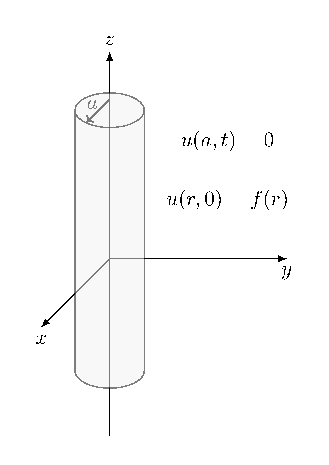
\includegraphics[scale=0.975]{Imagenes/plot_cilindro_Bessel_01.eps}
\end{figure}
\end{frame}
\begin{frame}
\frametitle{Orientación del cilindro}
Vemos que no importa la orientación del cilindro, ya sea que lo presentamos de manera horizontal o vertical, el punto importante es considerar que el eje $z$ \enquote{cruza} al cilindro por el centro.
\end{frame}

\subsection{Ecuación que modela}

\begin{frame}
\frametitle{Siguiente paso}
De acuerdo con lo que nos plantea el enunciado, la ecuación que debemos de ocupar, es la ecuación de calor:
\pause
\begin{align}
\pdv{u}{t} = \kappa \left( \pdv[2]{u}{r} + \dfrac{1}{r}  \, \pdv{u}{r} \right) \hspace{1.5cm} 0 < r < a, \hspace{0.5cm} t > 0
\label{eq:ecuacion_CilBessel_01}
\end{align}
\pause
junto con las condiciones:
\pause
\begin{align}
u(a, t) = 0 \hspace{2cm} u(r, 0) = f(r)
\label{eq:ecuacion_CilBessel_02}
\end{align}
\end{frame}
\begin{frame}
\frametitle{Consideración adicional}
Debemos de tomar en cuenta que la función $u(r, t)$ (solución) debe de ser acotada en todo el volumen del cilindro.
\end{frame}

\subsection{Resolviendo la ecuación}

\begin{frame}
\frametitle{Usando lo que hemos trabajado}
Tenemos una EDP lineal y homogénea, por lo que podemos apoyarnos con la técnica de \emph{separación de variables}.
\\
\bigskip
\pause
Como la distribución de temperatura no depende  de la parte angular $\theta$, así como del eje $z$, se simplifica el problema.
\end{frame}
\begin{frame}
\frametitle{Solución propuesta}
Se propone una solución del tipo:
\pause
\begin{align*}
u(r, t) = R(r) \, T(t)
\end{align*}
\pause
por lo que se calculan las derivadas parciales $u_{t}$, $u_{r}$ y $u_{rr}$, que vamos a sustituir en la ec. (\ref{eq:ecuacion_CilBessel_01}):
\end{frame}
\begin{frame}
\frametitle{Las derivadas parciales}
Se tiene entonces que:
\pause
\begin{align*}
u_{t} &= R(r) \, \ptilde{T}(t) \\[0.5em]
u_{r} &= \ptilde{R}(r) \, {T}(t) \\[0.5em]
u_{rr} &= \stilde{R}(r) \, {T}(t)
\end{align*}
que se sustituyen en la ecuación de calor.
\end{frame}
\begin{frame}
\frametitle{Ecuación de calor modificada}
Llegamos a:
\pause
\begin{align*}
R(r) \, \ptilde{T}(t) = \kappa \bigg[ \stilde{R}(r) \, {T}(t) + \dfrac{1}{r} \, \ptilde{R}(r) \, {T}(t) \bigg]
\end{align*}
\end{frame}
\begin{frame}
\frametitle{Ecuación de calor modificada}
Esta expresión la dividimos entre $R(r) \, T(t)$:
\pause
\begin{align*}
\dfrac{\ptilde{T}}{T} = \kappa \bigg[ \dfrac{\stilde{R}}{R} + \dfrac{1}{r} \, \dfrac{\ptilde{R}}{R} \bigg]
\end{align*}
\pause
simplificamos la expresión:
\pause
\begin{align*}
\dfrac{\stilde{R} + \dfrac{1}{r} \ptilde{R}}{R} = \dfrac{1}{\kappa} \, \dfrac{\ptilde{T}}{T}
\end{align*}
\end{frame}
\begin{frame}
\frametitle{Constante de separación}
Cada lado de la igualdad depende de una sola variable, al suponer que éstas son independientes entre sí, la única forma en la que se cumple la expresión, es que debe de ser igual a una constante.
\pause
\\
\bigskip
La constante de separación será: $-\lambda^{2}$.
\end{frame}
\begin{frame}
\frametitle{Constante de separación}
La constante de separación es:
\pause
\begin{align*}
\dfrac{\stilde{R} + \dfrac{1}{r} \ptilde{R}}{R} = \dfrac{1}{\kappa} \, \dfrac{\ptilde{T}}{T} = -\lambda^{2}
\end{align*}
\pause
Debemos de considerar la condición de frontera $u(a, t) = 0$:
\pause
\begin{align*}
R(a) \, T(t) = 0 \hspace{1cm} \Rightarrow \hspace{1cm} R(a) = 0
\end{align*}
\end{frame}
\begin{frame}
\frametitle{Sistema de dos EDO2H}
Llegamos a un sistema de dos EDO2H:
\pause
\begin{align}
\stilde{R}(r) + \dfrac{1}{r} \, \ptilde{R} + \lambda^{2} \, R(r) &= 0, \hspace{1.5cm} R(a) = 0 \label{eq:ecuacion_CilBessel_03} \\[0.5em]
\ptilde{T}(t) + \kappa \, \lambda^{2} \, T(t) &= 0 \label{eq:ecuacion_CilBessel_04}
\end{align}
\end{frame}

\section{Propiedades de la función de Bessel}
\frame{\tableofcontents[currentsection, hideothersubsections]}
\subsection{Identificando la ecuación}

\begin{frame}
\frametitle{Corresponencia con la ED de Bessel}
La ec. (\ref{eq:ecuacion_CilBessel_03}) que es la parte radial del problema:
\pause
\begin{align*}
\stilde{R}(r) + \dfrac{1}{r} \, \ptilde{R} + \lambda^{2} \, R(r) = 0
\end{align*}
\pause
es una ecuación de tipo Bessel:
\pause
\begin{align*}
\stilde{y} + \dfrac{1}{x} \, \ptilde{y} + \left( \lambda^{2} - \dfrac{\nu^{2}}{x^{2}} \right) \, y = 0
\end{align*}
\pause
Con $\nu = 0$.
\end{frame}
\begin{frame}
\frametitle{Solución general de la ED Bessel}
Sabemos que la solución general de la ED de Bessel es de la forma:
\pause
\begin{align*}
R(r) = C_{1} \, J_{0} (\lambda \, r) + C_{2} \, Y_{0} (\lambda \, r)
\end{align*}
con las constantes $C_{1}$ y $C_{2}$ por determinar.
\end{frame}

\subsection{Constricciones en el problema}

\begin{frame}
\frametitle{Funciones acotadas}
La función $R(r)$ debe de estar acotada en $r = 0$, por lo que se deduce que $C_{2} = 0$, ya que:
\pause
\begin{align*}
Y_{0}(0) \to \infty
\end{align*}
\pause
Por lo tanto:
\pause
\begin{align*}
R(r) = C_{1} \, J_{0}(\lambda \, r)
\end{align*}
\pause
como $R(a) = 0$, tenemos:
\pause
\begin{align*}
C_{1} \, J_{0} (\lambda \, a) = 0
\end{align*}
\end{frame}
\begin{frame}
\frametitle{Dos casos}
El caso trivial es cuando $C_{1} = 0$,\pause debiendo entonces considerar el caso no trivial: $C_{1} \neq 0$, así:
\pause
\begin{align}
J_{0} (\lambda \, a) = 0
\label{eq:ecuacion_CilBessel_05}
\end{align}
\end{frame}

\subsection{Soluciones a las EDO}

\begin{frame}
\frametitle{Solución a la ecuación radial}
Si $\lambda_{i} = 1, 2, \ldots$ son las raíces positivas de la ec. (\ref{eq:ecuacion_CilBessel_05}), se tiene que aparte del factor constante, las funciones:
\pause
\begin{align*}
R_{i}(r) = J_{0} (\lambda_{i} \, r) \hspace{1.5cm} i = 1, 2, \ldots
\end{align*}
son soluciones a la EDO2H radial, ec. (\ref{eq:ecuacion_CilBessel_03}).
\end{frame}
\begin{frame}
\frametitle{Solución a la ecuación en $t$}
Para los valores $\lambda$ considerados, la ec. (\ref{eq:ecuacion_CilBessel_04}), la parte temporal tiene las soluciones particulares:
\pause
\begin{align*}
T_{i} (t) = \exp(-\kappa \, \lambda_{i}^{2} \, t) \hspace{1.5cm} i = 1, 2, 3, \ldots
\end{align*}
\end{frame}
\begin{frame}
\frametitle{Solución completa}
La sucesión de funciones:
\pause
\begin{align*}
u_{i}(r, t) = J_{0} (\lambda_{i} \, r) \, \exp(-\kappa \, \lambda_{i}^{2} \, t) 
\end{align*}
\pause
satisfacen la ec. (\ref{eq:ecuacion_CilBessel_01}) así como la condición de frontera.
\end{frame}
\begin{frame}
\frametitle{Principio de superposición}
De acuerdo con el principio de superposición, la función:
\pause
\begin{align}
u(r, t) = \nsum_{i=1}^{\infty} C_{i} \, J_{0} (\lambda_{i} \, r) \, \exp(-\kappa \, \lambda_{i}^{2} \, t)
\label{eq:ecuacion_CilBessel_06}
\end{align}
\pause
también satisface a la ecuación de calor inicial y la CDF.
\end{frame}
\begin{frame}
\frametitle{Usando la condición inicial}
Ocupando la condición:
\pause
\begin{align*}
u(r, 0) = f(r)
\end{align*}
\pause
se obtiene la serie de Fourier-Bessel:
\pause
\begin{align}
f(r) = \nsum_{i=1}^{\infty} C_{i} \, J_{0}(\lambda_{i} \, r)
\label{eq:ecuacion_CilBessel_07}
\end{align}
\pause
quedando por determinar los coeficientes $C_{i}$. \pause Para obtener esos coeficientes, haremos un breve repaso sobre las series de Fourier-Bessel.
\end{frame}

\subsection{Series de Fourier-Bessel}

\begin{frame}
\frametitle{La serie de Fourier-Bessel}
Supongamos que una función $f(x)$ tiene un desarrollo convergente de la forma:
\pause
\begin{align}
f(x) = \nsum_{i=1}^{\infty} C_{i} \, J_{\nu} (\lambda_{i} \, x) \hspace{1.5cm} 0 < x < a
\label{eq:ecuacion_CilBessel_08}
\end{align}
donde los $\lambda_{i}$ con $i = 1, 2, \ldots$ son las raíces positivas de $J_{\nu} (\lambda \, a) = 0$
\end{frame}
\begin{frame}
\frametitle{Operando la función}
Multiplicamos ambos lados de la ec. (\ref{eq:ecuacion_CilBessel_08}) por $x \, J_{\nu}(\lambda_{j} \, x)$ con $j$ fijo, para luego integrar entre $0$ y $a$, suponiendo que la serie es integrable término a término, llegando a:
\pause
\begin{align*}
\int_{0}^{a} x \, f(x) \, J_{\nu}(\lambda_{j} \, x) \dd{x} = \nsum_{i=1}^{\infty} C_{i} \scaleint{6ex}_{\bs 0}^{a} x \, J_{\nu} (\lambda_{i} \, x) \, J_{\nu} (\lambda_{j} \, x) \dd{x}
\end{align*}
\pause
Para resolver la integral del lado derecho, habrá que emplear la propiedad de ortogonalidad de las funciones de Bessel.
\end{frame}
\begin{frame}
\frametitle{Ortogonalidad de las funciones de Bessel}
Sabemos que las funciones de Bessel cuentan con la propiedad de ortogonalidad, dada por la expresión:
\pause
\begin{align*}
\scaleint{6ex}_{\bs 0}^{a} x \, J_{\nu} (\lambda_{i} \, x) \, &J_{\nu} (\lambda_{j} \, x) \dd{x} = \\[1em]
&= \begin{cases}
0 & i \neq j \\
\dfrac{a^{2}}{2} \, J_{\nu+1}^{2} (\lambda_{i} \, a) & i = j, \hspace{0.5cm} i = 1, 2, \ldots
\end{cases}
\end{align*}
\end{frame}
\begin{frame}
\frametitle{Los coeficientes $C_{i}$}
Los coeficientes $C_{i}$ son:
\pause
\begin{eqnarray*}
\begin{aligned}
C_{i} &= \dfrac{\scaleint{6ex}_{\bs 0}^{a} x \, f(x) \, J_{\nu}(\lambda_{i} \, x) \dd{x}}{\scaleint{6ex}_{\bs 0}^{a} x \, J_{\nu}^{2} (\lambda_{i} \, x) \dd{x}} \hspace{1cm} i = 1, 2, \ldots \\[1em] \pause
&= \dfrac{\scaleint{6ex}_{\bs 0}^{a} x \, f(x) \, J_{\nu}(\lambda_{i} \, x) \dd{x}}{\dfrac{a^{2}}{2} \, J_{\nu+1}^{2} (\lambda_{i} \, a)} \hspace{1cm} i = 1, 2, \ldots
\end{aligned}
\end{eqnarray*}
\end{frame}
\begin{frame}
\frametitle{Los coeficientes $C_{i}$}
Los coeficientes $C_{i}$ quedan definidos por la expresión:
\pause
\begin{align*}
C_{i} = \dfrac{2}{a^{2}} \dfrac{\scaleint{6ex}_{\bs 0}^{a} x \, f(x) \, J_{\nu}(\lambda_{i} \, x) \dd{x}}{J_{\nu+1}^{2} (\lambda_{i} \, a)} \hspace{1cm} i = 1, 2, \ldots
\end{align*}
\pause
Con este resultado, ya podemos regresar al ejercicio y definir la solución completa al problema.
\end{frame}


\subsection*{Regresando a la solución}

\begin{frame}
\frametitle{La expresión para los $C_{i}$ del problema}
Con acuerdo a la manera en que se obtuvieron los coeficientes $C_{i}$ de una serie de Fourier-Bessel, para el problema del cilindro, se tiene que:
\pause
\begin{align}
C_{i} = \dfrac{2}{a^{2} \, J_{1}^{2} (\lambda_{i} \, a)} \scaleint{6ex}_{\bs 0}^{a} r \, f(r) \, J_{0}(\lambda_{i} \, r) \dd{r} \hspace{1cm} i = 1, 2, \ldots
\label{eq:ecuacion_Cil_Bessel_09}
\end{align}
\end{frame}
\begin{frame}
\frametitle{Solución completa}
La distribución de temperaturas en el cilindro viene dada por la expresión:
\pause
\begin{equation}
\begin{aligned}[b]
u(r, t) = \dfrac{2}{a^{2}} \nsum_{i=1}^{\infty} &\bigg[ \, \scaleint{6ex}_{\bs 0}^{a} \, r \, f(r) J_{0} (\lambda_{i} \, r) \dd{r} \bigg] \,\dfrac{J_{0} (\lambda_{i} \, r)}{J_{1}^{2} (\lambda_{i} \, a)} \times \\[1em]
&\times \exp( -\kappa \, \lambda_{i}^{2} \, t)
\end{aligned}
\label{eq:ecuacion_CilBessel10}
\end{equation}
donde la suma es tomada sobre todas las raíces positivas de la ec. (\ref{eq:ecuacion_CilBessel_05}) $\qed$.
\end{frame}
% \begin{frame}
% \frametitle{Problema opcional}
% Resolver el siguiente ejercicio es opcional, contabiliza para los ejercicios del tema, es decir, habrá $5$ ejercicios que deberán de resolverse, más este problema.
% \\
% \bigskip
% \pause
% Este ejercicio bien resuelto aportaría puntaje para la calificación
% \end{frame}

\begin{frame}
\frametitle{Modificando las condiciones del mismo problema}
Si se reemplaza la condición de que la superficie lateral del cilindro se mantiene a temperatura cero, por la condición de que a través de dicha superficie se transmite calor a una medio circundante que está a temperatura cero, es decir:
\pause
\begin{align*}
u_{r} (a, t) = - h \, u(a, t) \hspace{1.5cm} h \mbox{ constante}
\end{align*}
\end{frame}
\begin{frame}
\frametitle{Solución del problema}
Se puede demostrar (ejercicio moral) que la solución es:
\pause
\begin{align*}
u(r, t) &= \dfrac{2}{a^{2}} \nsum_{i=1}^{\infty} \dfrac{\lambda_{i}^{2}}{(\lambda_{i}^{2} {+} h^{2}) \, J_{0}^{2} (\lambda_{i} \, a)} \bigg[ \, \scaleint{6ex}_{\bs 0}^{a} \, r \, f(r) J_{0} (\lambda_{i} \, r) \dd{r} \bigg] \times \\[1em] 
&\times J_{0} (\lambda_{i} \, r) \exp( -\kappa \, \lambda_{i}^{2} \, t)    
\end{align*}
\end{frame}
\begin{frame}
\frametitle{Raíces positivas}
Donde la suma es tomada sobre todas las raíces positivas de la ecuación:
\pause
\begin{align*}
h \, J_{0} (\lambda \, a) + \lambda \, \ptilde{J}_{0} (\lambda \, a) = 0
\end{align*}
\end{frame}
\begin{frame}
\frametitle{Ejercicio a cuenta - 8}
%Ref. Arfken(2006) 11.2.7
Un cilindro circular recto tiene un potencial electrostático $\psi (\rho, \varphi)$ en los extremos, mientras que el potencial en la superficie curva del cilindro es cero.
\end{frame}

\begin{frame}
\frametitle{Ejercicio a cuenta - 8}
Calcula el potencial en los puntos interiores del cilindro.
\\
\bigskip
Nota: Elige debidamente el sistema coordenado para que ajustes la dependencia de $z$ y explotes al máximo la simetría del potencial.
\end{frame}
    

\end{document}